\documentclass{mimosis}

\usepackage{metalogo}

%%%%%%%%%%%%%%%%%%%%%%%%%%%%%%%%%%%%%%%%%%%%%%%%%%%%%%%%%%%%%%%%%%%%%%%%
% Some of my favourite personal adjustments
%%%%%%%%%%%%%%%%%%%%%%%%%%%%%%%%%%%%%%%%%%%%%%%%%%%%%%%%%%%%%%%%%%%%%%%%
%
% These are the adjustments that I consider necessary for typesetting
% a nice thesis. However, they are *not* included in the template, as
% I do not want to force you to use them.

% This ensures that I am able to typeset bold font in table while still aligning the numbers
% correctly.
\usepackage{etoolbox}

% Add todonotes for writing process
\usepackage{todonotes}

% use libertinus font 
\usepackage{libertinus}

% for tables 
\usepackage{tabularray}
% for useful symbols
\usepackage{gensymb}

% for compact lists
\usepackage{enumitem}

% \usepackage{subfig}

%%%%%%%%%%%%%%%%%%%%%%%%%%%%%%%%%%%%%%%%%%%%%%%%%%%%%%%%%%%%%%%%%%%%%%%%
% Hyperlinks & bookmarks
%%%%%%%%%%%%%%%%%%%%%%%%%%%%%%%%%%%%%%%%%%%%%%%%%%%%%%%%%%%%%%%%%%%%%%%%

\usepackage[%
  colorlinks = true,
  citecolor  = RoyalBlue,
  linkcolor  = RoyalBlue,
  urlcolor   = RoyalBlue,
  unicode,
  ]{hyperref}

\usepackage{bookmark}

% for better footnotes
\usepackage{cleveref}
\crefformat{footnote}{#2\footnotemark[#1]#3}
%%%%%%%%%%%%%%%%%%%%%%%%%%%%%%%%%%%%%%%%%%%%%%%%%%%%%%%%%%%%%%%%%%%%%%%%
% Bibliography
%%%%%%%%%%%%%%%%%%%%%%%%%%%%%%%%%%%%%%%%%%%%%%%%%%%%%%%%%%%%%%%%%%%%%%%%
%
% I like the bibliography to be extremely plain, showing only a numeric
% identifier and citing everything in simple brackets. The first names,
% if present, will be initialized. DOIs and URLs will be preserved.

\usepackage[%
  autocite     = plain,
  backend      = biber,
  doi          = true,
  url          = false,
  giveninits   = true,
  hyperref     = true,
  maxbibnames  = 99,
  maxcitenames = 2,
  sortcites    = true,
  style        = numeric,
  ]{biblatex}

%%%%%%%%%%%%%%%%%%%%%%%%%%%%%%%%%%%%%%%%%%%%%%%%%%%%%%%%%%%%%%%%%%%%%%%%
% Some adjustments to make the bibliography more clean
%%%%%%%%%%%%%%%%%%%%%%%%%%%%%%%%%%%%%%%%%%%%%%%%%%%%%%%%%%%%%%%%%%%%%%%%
%
% The subsequent commands do the following:
%  - Removing the month field from the bibliography
%  - Fixing the Oxford commma
%  - Suppress the "in" for journal articles
%  - Remove the parentheses of the year in an article
%  - Delimit volume and issue of an article by a colon ":" instead of
%    a dot ""
%  - Use commas to separate the location of publishers from their name
%  - Remove the abbreviation for technical reports
%  - Display the label of bibliographic entries without brackets in the
%    bibliography
%  - Ensure that DOIs are followed by a non-breakable space
%  - Use hair spaces between initials of authors
%  - Make the font size of citations smaller
%  - Fixing ordinal numbers (1st, 2nd, 3rd, and so) on by using
%    superscripts

% Remove the month field from the bibliography. It does not serve a good
% purpose, I guess. And often, it cannot be used because the journals
% have some crazy issue policies.
\AtEveryBibitem{\clearfield{month}}
\AtEveryCitekey{\clearfield{month}}

% Fixing the Oxford comma. Not sure whether this is the proper solution.
% More information is available under [1] and [2].
%
% [1] http://tex.stackexchange.com/questions/97712/biblatex-apa-style-is-missing-a-comma-in-the-references-why
% [2] http://tex.stackexchange.com/questions/44048/use-et-al-in-biblatex-custom-style
%
\AtBeginBibliography{%
  \renewcommand*{\finalnamedelim}{%
    \ifthenelse{\value{listcount} > 2}{%
      \addcomma
      \addspace
      \bibstring{and}%
    }{%
      \addspace
      \bibstring{and}%
    }
  }
}

% Suppress "in" for journal articles. This is unnecessary in my opinion
% because the journal title is typeset in italics anyway.
\renewbibmacro{in:}{%
  \ifentrytype{article}
  {%
  }%
  % else
  {%
    \printtext{\bibstring{in}\intitlepunct}%
  }%
}

% Remove the parentheses for the year in an article. This removes a lot
% of undesired parentheses in the bibliography, thereby improving the
% readability. Moreover, it makes the look of the bibliography more
% consistent.
\renewbibmacro*{issue+date}{%
  \setunit{\addcomma\space}
    \iffieldundef{issue}
      {\usebibmacro{date}}
      {\printfield{issue}%
       \setunit*{\addspace}%
       \usebibmacro{date}}%
  \newunit}

% Delimit the volume and the number of an article by a colon instead of
% by a dot, which I consider to be more readable.
\renewbibmacro*{volume+number+eid}{%
  \printfield{volume}%
  \setunit*{\addcolon}%
  \printfield{number}%
  \setunit{\addcomma\space}%
  \printfield{eid}%
}

% Do not use a colon for the publisher location. Instead, connect
% publisher, location, and date via commas.
\renewbibmacro*{publisher+location+date}{%
  \printlist{publisher}%
  \setunit*{\addcomma\space}%
  \printlist{location}%
  \setunit*{\addcomma\space}%
  \usebibmacro{date}%
  \newunit%
}

% Ditto for other entry types.
\renewbibmacro*{organization+location+date}{%
  \printlist{location}%
  \setunit*{\addcomma\space}%
  \printlist{organization}%
  \setunit*{\addcomma\space}%
  \usebibmacro{date}%
  \newunit%
}

% Display the label of a bibliographic entry in bare style, without any
% brackets. I like this more than the default.
%
% Note that this is *really* the proper and official way of doing this.
\DeclareFieldFormat{labelnumberwidth}{#1\adddot}

% Ensure that DOIs are followed by a non-breakable space.
\DeclareFieldFormat{doi}{%
  \mkbibacro{DOI}\addcolon\addnbspace
    \ifhyperref
      {\href{http://dx.doi.org/#1}{\nolinkurl{#1}}}
      %
      {\nolinkurl{#1}}
}

% Use proper hair spaces between initials as suggested by Bringhurst and
% others.
\renewcommand*\bibinitdelim {\addnbthinspace}
\renewcommand*\bibnamedelima{\addnbthinspace}
\renewcommand*\bibnamedelimb{\addnbthinspace}
\renewcommand*\bibnamedelimi{\addnbthinspace}

% Make the font size of citations smaller. Depending on your selected
% font, you might not need this.
\usepackage{relsize}
\renewcommand*{\citesetup}{%
  \biburlsetup
  \relsize{-.5}%
}

\DeclareLanguageMapping{english}{english-mimosis}

% Make hyperlinks extend to the author name if `\textcite` is being used
% instead of another cite command.

\DeclareFieldFormat{citehyperref}{%
  % Need this to avoid nested links
  \DeclareFieldAlias{bibhyperref}{noformat}%
  \bibhyperref{#1}%
}

\DeclareFieldFormat{textcitehyperref}{%
  % Need this to avoid nested links
  \DeclareFieldAlias{bibhyperref}{noformat}%
  \bibhyperref{%
    #1%
    \ifbool{cbx:parens}
      {\bibcloseparen\global\boolfalse{cbx:parens}}
      {}%
    }%
}

\savebibmacro{cite}
\savebibmacro{textcite}

\renewbibmacro*{cite}{%
  \printtext[citehyperref]{%
    \restorebibmacro{cite}%
    \usebibmacro{cite}}%
}

\renewbibmacro*{textcite}{%
  \ifboolexpr{
    ( not test {\iffieldundef{prenote}} and
      test {\ifnumequal{\value{citecount}}{1}} )
    or
    ( not test {\iffieldundef{postnote}} and
      test {\ifnumequal{\value{citecount}}{\value{citetotal}}} )
  }%
  {\DeclareFieldAlias{textcitehyperref}{noformat}}
  {}%
  \printtext[textcitehyperref]{%
    \restorebibmacro{textcite}%
    \usebibmacro{textcite}}%
}

\addbibresource{zotero_lib.bib}
\addbibresource{custom_references.bib}

%%%%%%%%%%%%%%%%%%%%%%%%%%%%%%%%%%%%%%%%%%%%%%%%%%%%%%%%%%%%%%%%%%%%%%%%
% Fonts
%%%%%%%%%%%%%%%%%%%%%%%%%%%%%%%%%%%%%%%%%%%%%%%%%%%%%%%%%%%%%%%%%%%%%%%%

% change font for headings 

% set sans font to libertinus sans
% \renewcommand{\sfdefault}{Libertinus Sans}
% \titleformat*{\section}{\Large\sffamily}
% \titleformat*{\subsection}{\large\sffamily}
% \titleformat*{\subsubsection}{\normalsize\sffamily}


% set main font to libertinus Serif
% \setmainfont{Libertinus Serif}

% \setsansfont{IBM Plex Sans}
% \setmonofont{IBM Plex Mono}
% \ifxetexorluatex
%   \usepackage{unicode-math}
%   \setmainfont{Cambria}
%   \setmathfont{Cambria Math}
% 
%   % Load some missing symbols from another font.
%   \setmathfont{STIX Two Math}[%
%     range = {
%       \sharp,
%       \natural,
%       \flat,
%       \clubsuit,
%       \spadesuit,
%       \checkmark
%     }
%   ]
%   \setmonofont[Scale=MatchLowercase]{Source Code Pro}
% \else
%   \usepackage[lf]{ebgaramond}
%   \usepackage[oldstyle,scale=0.7]{sourcecodepro}
%   \singlespacing
% \fi

\newacronym[description={Principal component analysis}]{PCA}{PCA}{principal component analysis}
\newacronym[description={Empirical Orthogonal Functions}]{EOF}{EOF}{empirical orthogonal functions}
\newacronym                                            {SNF}{SNF}{Smith normal form}
\newacronym[description={Topological data analysis}]   {TDA}{TDA}{topological data analysis}
\newacronym                                            {GCM}{GCM}{Global Coupled Model}

\newglossaryentry{LaTeX}{%
  name        = {\LaTeX},
  description = {A document preparation system},
  sort        = {LaTeX},
}

\newglossaryentry{Real numbers}{%
  name        = {$\real$},
  description = {The set of real numbers},
  sort        = {Real numbers},
}

\makeindex
\makeglossaries

%%%%%%%%%%%%%%%%%%%%%%%%%%%%%%%%%%%%%%%%%%%%%%%%%%%%%%%%%%%%%%%%%%%%%%%%
% Custom Commands
%%%%%%%%%%%%%%%%%%%%%%%%%%%%%%%%%%%%%%%%%%%%%%%%%%%%%%%%%%%%%%%%%%%%%%%%

\newcommand{\citeauthorwork}[1]{\citeauthor{#1} \cite{#1}}

%%%%%%%%%%%%%%%%%%%%%%%%%%%%%%%%%%%%%%%%%%%%%%%%%%%%%%%%%%%%%%%%%%%%%%%%
% Ordinals
%%%%%%%%%%%%%%%%%%%%%%%%%%%%%%%%%%%%%%%%%%%%%%%%%%%%%%%%%%%%%%%%%%%%%%%%

\makeatletter
\@ifundefined{st}{%
  \newcommand{\st}{\textsuperscript{\textup{st}}\xspace}
}{}
\@ifundefined{rd}{%
  \newcommand{\rd}{\textsuperscript{\textup{rd}}\xspace}
}{}
\@ifundefined{nd}{%
  \newcommand{\nd}{\textsuperscript{\textup{nd}}\xspace}
}{}
\makeatother

\renewcommand{\th}{\textsuperscript{\textup{th}}\xspace}

% make only sections and chapters appear in TOC 
\setcounter{tocdepth}{1}
%%%%%%%%%%%%%%%%%%%%%%%%%%%%%%%%%%%%%%%%%%%%%%%%%%%%%%%%%%%%%%%%%%%%%%%%
%  Actual Document
%%%%%%%%%%%%%%%%%%%%%%%%%%%%%%%%%%%%%%%%%%%%%%%%%%%%%%%%%%%%%%%%%%%%%%%%


\begin{document}


\frontmatter
  
\newcommand{\titleOfThesis}{An interesting title about, EOF, Wind, Humidity and Climate}
\newcommand{\kindOfThesis}{Masterarbeit} % Bachelor or Master Thesis

\newcommand{\myuniversity}{Universität Leipzig}
\newcommand{\myuni}{Universität Leipzig} % short affiliation of the OvGU
\newcommand{\myunistreet}{Augustusplatz 10}
\newcommand{\myunizipcity}{04109 Leipzig, Germany}
\newcommand{\myschool}{Fakultät für Mathematik und Informatik}  % German
\newcommand{\mydepartment}{Institut für Informatik}
\newcommand{\myfirstname}{Denis}
\newcommand{\mylastname}{Streitmatter}
\newcommand{\mybirthdate}{30.\ December 1997}
\newcommand{\mybirthplace}{Kösching}

% infai/kilt info
\newcommand{\mycompany}{Institut für Angewandte Informatik}
\newcommand{\myworkinggroup}{KILT}
\newcommand{\mycompanystreet}{Goerdelerring 9}
\newcommand{\mycompanyzipcity}{04109 Leipzig, Germany}


\newcommand{\mydegree}{B.\ Sc.\ Computer Science}
\newcommand{\myplace}{Leipzig}
\newcommand{\myyear}{2021}

\begin{titlepage}
  \begin{center}
  {\LARGE \textbf{\myuniversity}}\\[5mm]
% \begin{figure*}[h]
% \hbox{}\hfill
% \begin{minipage}[t]{9cm}
%     		 \centering
%     		 
\includegraphics[width=4cm]{logos/uni-leipzig-logo.png}
% \end{minipage}
% \hfill\hbox{}
% \end{figure*}
  {\Large \myschool}\\
  {\large \mydepartment}\\[20mm]
		%{\large\bf \titleOfThesis}\\[10mm]
		{\Large\textbf \titleOfThesis}\\[10mm]
    {\LARGE \kindOfThesis}\\[10mm]
  %{\small Author:}\\[1mm]
  %{\large \myfirstname~\mylastname}\\[5mm]
  %{\small \today}\\[15mm]
  
  
% Needs to fit: http://studium.fmi.uni-leipzig.de/fileadmin/Studienbuero/documents/Formulare/Deckblatt_Dipl_BSc_MSc_Arbeit_.rtf
    
    
\vspace{5cm}
% \begin{tabular}{p{.6\textwidth}p{.5\textwidth}}
%     \multicolumn{1}{l}{submitted at \today}  & \multicolumn{1}{r}{submitted by} \\[3mm]
%     & \multicolumn{1}{r}{{\large \myfirstname~\mylastname}} \\
%     & \multicolumn{1}{r}{Informatik Bsc.}
% \end{tabular}




%   \vspace{1cm}
%   \renewcommand{\arraystretch}{.9}
%   \begin{tabular}{cc}
% 	\multicolumn{2}{c}{\small Advisers:} \\[1mm]
% 	{\small Supervisor} & {\small Supervisor} \\
% 	{\large Johannes Frey, M.Sc.} & {\large Dr.-Ing. Sebastian Hellmann} \\[2mm]
% 	{\small \myworkinggroup} 			 & {\small \myworkinggroup} \\
% 	{\small \mycompany} 			 & {\small \mycompany} 	\\
% 	{\small \mycompanystreet} 		 & {\small \mycompanystreet} \\
% 	{\small \myunizipcity}		 & {\small \myunizipcity} 
%   \end{tabular}
  
		\renewcommand{\arraystretch}{1}
  \end{center}
  
Leipzig, Mai 2024\hfill vorgelegt von \\[3mm]
\hspace*{\fill} {\large \myfirstname~\mylastname}\\
\hspace*{\fill} Studiengang Master Informatik

\vspace{1cm}

{\large \textbf{Betreuende Hochschullehrer:}}

{\large Dr.-Ing. Sebastian Hellmann }\\
\mycompany/KILT

{\large Johannes Frey, M.Sc. }\\
\mycompany/KILT

{\large Dr. Eric Peukert}\\
Abteilung Datenbanken Universität Leipzig
%  \vspace*{5cm}
%  \makeatletter
%  \begin{center}
%    \begin{Huge}
%      \@title
%    \end{Huge}\\[0.1cm]
%    %
%    \begin{Large}
%      \@subtitle
%    \end{Large}\\
%    %
%    \emph{by}\\
%    \@author  \mydegree
%    %
%    \vfill
%    A document submitted in partial fulfillment
%    of the requirements for the degree of\\
%    \emph{Technical Report}\\
%    at\\
%    \textsc{Miskatonic University}
%  \end{center}
  \makeatother
\end{titlepage}

\newpage
\null
\thispagestyle{empty}
\newpage

  %\begin{titlepage}
%\thispagestyle{titlepage}
%% Definitions for the title page
\newcommand{\titleOfThesis}{Design and Implementation of DBpedia Archivo - an Augmented Ontology Archive}
\newcommand{\kindOfThesis}{Bachelorarbeit} % Bachelor or Master Thesis
%\newcommand{\submission}{??.\ Monat 20??}  % German date of the thesis submission
%\newcommand{\colloquium}{??.\ Monat 20??} % German date of the dissertation colloquium

\newcommand{\myuniversity}{Universität Leipzig}
\newcommand{\myuni}{Universität Leipzig} % short affiliation of the OvGU
\newcommand{\myunistreet}{Augustusplatz 10}
\newcommand{\myunizipcity}{04109 Leipzig, Germany}
\newcommand{\myschool}{Fakultät für Mathematik und Informatik}  % German
\newcommand{\mydepartment}{Institut für Informatik}
\newcommand{\myfirstname}{Denis}
\newcommand{\mylastname}{Streitmatter}
\newcommand{\mybirthdate}{30.\ December 1997}
\newcommand{\mybirthplace}{Kösching}

% infai/kilt info
\newcommand{\mycompany}{Institut für Angewandte Informatik}
\newcommand{\myworkinggroup}{KILT}
\newcommand{\mycompanystreet}{Goerdelerring 9}
\newcommand{\mycompanyzipcity}{04109 Leipzig, Germany}


\newcommand{\mydegree}{B.\ Sc.\ Computer Science}
%\newcommand{\firstadvisor}{Prof.\ Dr.\ First Last1}
%\newcommand{\secondadvisor}{Prof.\ Dr.\ First Last2}
%\newcommand{\thirdadvisor}{Prof.\ Dr.\ First Last3}
\newcommand{\myplace}{Leipzig}
\newcommand{\myyear}{2021}
  \begin{center}
  {\LARGE \textbf{\myuniversity}}\\[5mm]
\begin{figure*}[h]
\hbox{}\hfill
\begin{minipage}[t]{9cm}
    		 \centering
    		 
\includegraphics[width=4cm]{logos/uni-leipzig-logo.png}
\end{minipage}
\hfill\hbox{}
\end{figure*}
  {\Large \myschool}\\
  {\large \mydepartment}\\[20mm]
		%{\large\bf \titleOfThesis}\\[10mm]
		{\Large\textbf \titleOfThesis}\\[10mm]
    {\LARGE \kindOfThesis}\\[10mm]
  %{\small Author:}\\[1mm]
  %{\large \myfirstname~\mylastname}\\[5mm]
  %{\small \today}\\[15mm]
  
  
% Needs to fit: http://studium.fmi.uni-leipzig.de/fileadmin/Studienbuero/documents/Formulare/Deckblatt_Dipl_BSc_MSc_Arbeit_.rtf
    
    
\vspace{5cm}
% \begin{tabular}{p{.6\textwidth}p{.5\textwidth}}
%     \multicolumn{1}{l}{submitted at \today}  & \multicolumn{1}{r}{submitted by} \\[3mm]
%     & \multicolumn{1}{r}{{\large \myfirstname~\mylastname}} \\
%     & \multicolumn{1}{r}{Informatik Bsc.}
% \end{tabular}




%   \vspace{1cm}
%   \renewcommand{\arraystretch}{.9}
%   \begin{tabular}{cc}
% 	\multicolumn{2}{c}{\small Advisers:} \\[1mm]
% 	{\small Supervisor} & {\small Supervisor} \\
% 	{\large Johannes Frey, M.Sc.} & {\large Dr.-Ing. Sebastian Hellmann} \\[2mm]
% 	{\small \myworkinggroup} 			 & {\small \myworkinggroup} \\
% 	{\small \mycompany} 			 & {\small \mycompany} 	\\
% 	{\small \mycompanystreet} 		 & {\small \mycompanystreet} \\
% 	{\small \myunizipcity}		 & {\small \myunizipcity} 
%   \end{tabular}
  
		\renewcommand{\arraystretch}{1}
  \end{center}
  
Leipzig, März 2021\hfill vorgelegt von \\[3mm]
\hspace*{\fill} {\large \myfirstname~\mylastname}\\
\hspace*{\fill} Studiengang Bachelor Informatik

\vspace{1cm}

{\large \textbf{Betreuende Hochschullehrer:}}

{\large Dr.-Ing. Sebastian Hellmann }\\
\mycompany/KILT

{\large Johannes Frey, M.Sc. }\\
\mycompany/KILT

{\large Dr. Eric Peukert}\\
Abteilung Datenbanken Universität Leipzig
  
\end{titlepage}

\thispagestyle{empty}
\vspace*{\fill}
\begin{minipage}{.95\textwidth}
\textbf{\mylastname,\myfirstname}\newline
\emph{\titleOfThesis}\newline
\kindOfThesis, \myuni \newline
\myplace, \myyear.
\end{minipage}

\cleardoublepage

% =============================================================================

%%%%%%%%%%%%%%%%%%%%%%%%%%%%%%%%%%%%%%%%%%%%%%%%%%%%%%%%%%%%%%%%%%%%%%%%%%%%%
%%% Inhaltsverzeichnis
%%%%%%%%%%%%%%%%%%%%%%%%%%%%%%%%%%%%%%%%%%%%%%%%%%%%%%%%%%%%%%%%%%%%%%%%%%%%%

\setcounter{tocdepth}{2}
\tableofcontents

%\addcontentsline{toc}{chapter}{Abbildungsverzeichnis}
%\listoffigures

%\addcontentsline{toc}{chapter}{Tabellenverzeichnis}
%\listoftables

%\addcontentsline{toc}{chapter}{Algorithmenverzeichnis}
%\listofalgorithms
%\todo{Anleitung Algorithmen schreiben: \url{http://en.wikibooks.org/wiki/LaTeX/Algorithms}}

\cleardoublepage
% =============================================================================

\phantomsection
\section*{Abstract}
\addcontentsline{toc}{chapter}{Abstract}
Over the last years, a huge amount of work has been done to improve the ability of machines to utilize data on the Web. One approach is the Semantic Web, using ontologies as a way to make the knowledge of a domain machine-usable. Even though many ontologies were developed and published, a unified system to handle those has not surfaced, leaving consumers as well as publishers to deal with many uncertainties and challenges. 

This thesis presents DBpedia Archivo, an augmented ontology archive. It discovers, crawls, versions, and archives ontologies available on the Web. Each version of them is persisted on the DBpedia Databus. Additionally, Archivo augments the ontologies with different tests and features. 
The goals of Archivo are to provide a backup service for ontology-versions as well as to encourage publishers to follow best practices. 
For this Archivo rates the ontologies with a star system, making problems visible at a glance. A comparison to existing, similar systems is given.

\cleardoublepage
% =============================================================================


%\thispagestyle{plain}
%\phantom{.}
%\vspace{70mm}

%\begin{center}
%	\todo[inline]{This section is optional! It is basically an motivational cite for this work as it can be found in many books. Example is provided}
%	\textit{
%		\vspace{0.5cm}
%		The validation of clustering structures is \\
%		the most difficult and frustrating part of cluster analysis. \\ 
%		\vspace{0.5cm}
%		Without a strong effort in this direction, \\
%		cluster analysis will remain a black art 
%		accessible only to those \\
%		true believers who have experience and great courage.}
%\end{center}
%\begin{flushright}
%	\citet{Jain1988}
%	Anil K. Jain and Richard C. Dubes
%\end{flushright}

%\uselengthunit{mm}
%textwidth=\printlength{\textwidth}\\
%textheight=\printlength{\textheight}\\
%top=\printlength{\top}\\

%\cleardoublepage
% =============================================================================


%\thispagestyle{plain}
%\section*{Acknowledgements}
%\todo[inline]{This section is optional!}

%\cleardoublepage
% =============================================================================


  \begin{center}
  \textsc{Abstract}
\end{center}
%
\noindent
%
Scientific documents often use \LaTeX{} for typesetting. While numerous
packages and templates exist, it makes sense to create a new one. Just
because.


  \tableofcontents

\mainmatter
  \chapter{Introduction and Motivation}
\label{ch:introduction}


\section{Motivation}
\label{sec:motivation}





\section{Structure of this Thesis}


  
\chapter{Basics}
\label{ch:basics}

% This section should explain the basic math to understand the aforementioned topics, not that much needed but still needs to be there.

\section{Sampled Data, Grids and (Uncertain) Fields}
\label{sec:uncertainfields}

The goal of this section is to give insights into the structure of scientific (sampled) data, grids, interpolation, and (uncertain) fields. 
Especially the first parts of this section are largely based on the work of \citeauthorwork{telea2014data}, for a more extensive introduction please refer to it. 

\subsection{Sampled Data, Grids and Interpolation}

In general, data can be classified into two categories: intrinsically continuous or intrinsically discrete data. 
The latter refers to data such as websites, texts, source code, images or any other type of record. 
The first on the other hand usually stems from nature and is measured in physical units like $kg$, $\frac{m}{s}$ or similar.
Continuous data conforms to the Cauchy-Criterion (also called the $\epsilon - \delta$-Criterion), which essentially states that a function $f(x)$ is uniformly continuous if, for any small amount $\epsilon$ you choose, you can find a small distance $\delta$ such that whenever two points are within $\delta$ of each other, their function values are within $\epsilon$ of each other (see \cite{telea2014data} for the mathematical definition). 
Continuous data can be mathematically represented as a function in the form of \cite{telea2014data}:

\begin{equation}
  f: D \rightarrow C
  \label{eq:continous data}
\end{equation}

With $D \subset \mathbb{R}^d$ and $C \subset \mathbb{R}^c$. 
In this case the function is called a d-dimensional, c-valued function, which means it maps from its original function domain $D$ to values in the $C$ domain. 
Functions with $c=1$ are called Scalar Fields, assigning every position in the function domain a single scalar attribute $x \in \mathbb{R}$. 
Vector Fields ($c=2$ or $c=3$) on the other hand assign every position a vector in the form of $(x_1, x_2) \in \mathbb{R}^2$ or $(x_1, x_2, x_3) \in \mathbb{R}^3$, which can (but does not have to) depend on the original function domain. 
There are also fields related to higher dimensions (Tensor fields), but they are beyond the scope of this Thesis. 

Although this kind of data is continuous in the real world, its computational representation is nearly always discrete. 
The reason for this is that it is a) hard to achieve continuous data and b) many mathematical operations (e.g. filtering, denoising, rendering) are hard to perform on continuous data. 
According to \citeauthorwork{telea2014data}, this is called \textit{sampled data} and could come from e.g. measurements or computer simulations. 
The sampled data can then be used to reconstruct the original, continuous dataset by using interpolation. 
Therefor, when a field is mentioned in this Thesis, it usually refers to such an approximation of a continuous field like in Equation~\ref{eq:continous data}. 


Interpolation usually uses the structure of data, which is mostly called a \textit{grid} (or sometimes mesh). 
A grid is a subdivision of the original function domain $D$ into a non\--overlapping collection of cells, which in turn are spanned by vertices, which are the sample points of the discretization of the continuous field.  
There are multiple ways of defining grids (e.g. rectilinear, structured, unstructured, see Figure~\ref{fig:grid types}) and cells (examples for 2D: line, triangle, quad, hexahedron), but for the sake of brevity this section only introduces the grid applied by the dataset used for this Thesis: The uniform grid. 

\begin{figure}
  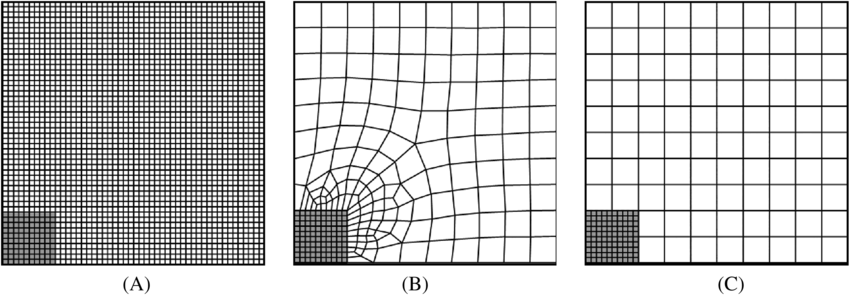
\includegraphics[width=0.95\textwidth]{figures/grid-types.png}
  \caption{Different types of Grids: A) Uniform Grid, B) unstructured grid, and C) no-conforming grid from \cite{kaltenbacher_nonconforming_2022}}
  \label{fig:grid types}
\end{figure}


A uniform grid is essentially an axis-aligned box spanning over the original function domain $D$. 
The extent of the box can be described as a list of $d$ pairs:

\begin{equation}
  ((m_1, M_1),\dots,(m_d, M_d)), (m_i, M_i) \in \mathbb{R}^2, m_i < M_i
  \label{eq:uniform grid coordinates}
\end{equation}

$(m_i, M_i)$  make up the lower and upper limit of the extent in each axis' direction. 
The sample points are then uniformly distributed along the axis with a given distance $\delta_i$ depending on the axis and all sample points $p_i$ can be described with: 

\begin{equation}
  p_i = (m_1 + n_i\delta_i,\dots, m_d + n_d\delta_d), n_1, \dots, n_d \in \mathbb{N}
  \label{eq:smaple point uniform grid}
\end{equation}

Therefor, every sample point can be described by its integer coordinates $n_1, \dots, n_d$. 
The number of sample points on axis $i$ is then $N_i = 1 + (M_i - m_i)/\delta_i$, and the set $(N_1, \dots, N_d)$ is often called the \textit{shape} of the uniform grid.   
The benefits of using uniform grids are the very low storage requirements ($3d$ floating point numbers, regardless of its size) and its simple implementation. 
Drawbacks are mainly that uniform grids do not represent all use-cases well or require an unnecessary high density to do so. 


Interpolation is the process of reconstructing the continuous data $f$ (Equation~\ref{eq:continous data}) from sampled points $p_i$ and associated values $f_i$. 
In general, there are multiple ways of interpolating, for example using by using \textit{nearest-neighbor interpolation}, assigning each point the value of the closest cell center. 
While this is computationally efficient, it is a staircase-like, discontinuous approximation of the original data. 
A better, continuous approach is linear interpolation, which interpolates the value of a point $x \in D$ based on the surrounding cell. 
But since interpolation is handled at the very last, visualization step (and handled by libraries), the full mathematical description (and other interpolation ideas) are out of the scope of this Thesis, but are detailed in \citeauthorwork{telea2014data}. 

\subsection{Map Projections}
\label{sec:map projections}

Regarding the original function dimension $d$ of the field $f$ described in Equation~\ref{eq:continous data}, there is a subtle but important distinction: the \textit{geometrical dimension} versus the \textit{topological dimension}. 
The geometrical dimension refers to the dimension of space $D$ is embedded in ($d$), while the topological dimension refers to the actual function domain $D$ itself, which is $s\leq d$ \cite{telea2014data}.
The difference is best illustrated with the example of the application in this Thesis: simulating earth's surface. 
Since the earth is a three-dimensional object, and also the earths surface is (approximately) a sphere's surface, the geometrical dimension of such datasets is $d=3$. 
But since the earths surface can be is a (curved) plane, the topological dimension of such datasets is $s=2$, which is also the reason why it is enough to access any gridpoint on earths with two coordinates: \textit{latitude} (lat), referring to the degrees on the north-south axis, and \textit{longitude} (lon), referring to degrees on the east-west axis.
Typically, since the topological dimension is the more relevant one, it is referred to as the \textit{dataset dimension}, while the geometrical dimension is mostly assumed to be three. \cite{telea2014data}

\begin{figure}[htp]
  \begin{center}
    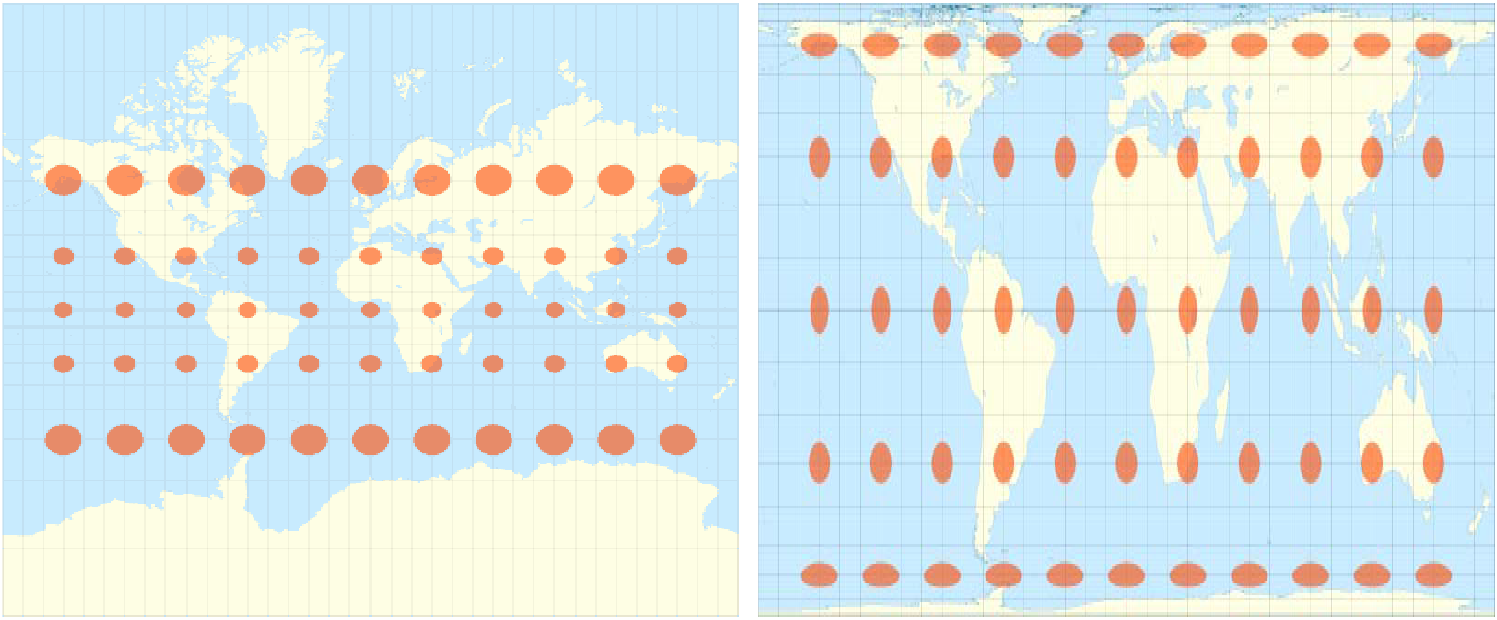
\includegraphics[width=0.95\textwidth]{figures/tissot-map-projections.png}
  \end{center}
  \caption{Two different map projections with different kinds of warping, depending on the map projection. The amount of warping is indicated by Tissot’s indicatrices (orange circles). Left: Mercator Projection, Right: Lambert Equal-Area Projection \cite{ghaderpour_map_2014}}\label{fig:tissot map projections}
\end{figure}


Unfortunately, this requires the mapping of a 2D paper plane to a 2D sphere surface, which is topologically impossible (without distortions) \cite{vietinghoffdiss}.
Therefor, numerous different map projections were invented, which all have a different kind of distortion in different geographical places. 
Figure~\ref{fig:tissot map projections} shows two distinct projections, both with their own advantages and disadvantages. 
As pointed out by \citeauthorwork{vietinghoffdiss}, a different map projections may fit the area of interest better, the Mercator projection in Figure~\ref{fig:tissot map projections} (left) is still chosen for this thesis, due to limitations in the employed map projections library (see Section~\ref{sec:vis_analysis}). 
This distortion also plays a role in calculations with uniform lon/lat-grids, since coordinates in the far north (and south) are vastly overrepresented, because they actually refer to a far smaller portion of the earth's surface than data near the equator (see Section~\ref{sec:eof} for geographical weighting). 


\subsection{Uncertain Fields}

% Explain uncertain fields and ensembles from \cite{vietinghoffdiss, pothkow2015modeling}

As already mentioned, the results of GCMs are often multiple simulations. 
Mathematically, this is defined as an \textit{uncertain} or \textit{random field}. 
Since all fields used in this Thesis are scalar fields, we will define uncertain fields only for those. 
Let's assume $s : D \rightarrow \mathbb{R}$ is a scalar field, associating a value  with every point in $D$. 
As mentioned in the previous section, such fields are usually approximated using $n$ sample points in a grid $(x_1,\dots, x_n) \in D^n$ and their associated scalar values, represented in a vector $(s_1,\dots,s_n) \in \mathbb{R}^n$ ($s_i$ is the scalar value at grid point $x_i$).
This being a \enquote{normal} (or rather deterministic) scalar field, an uncertain scalar has no concrete given values $s_i$ but follows an unknown probability density \cite{vietinghoffdiss}, which is illustrated in Figure~\ref{fig:uncertain field example}. 


\begin{figure}[htb]
  \begin{center}
    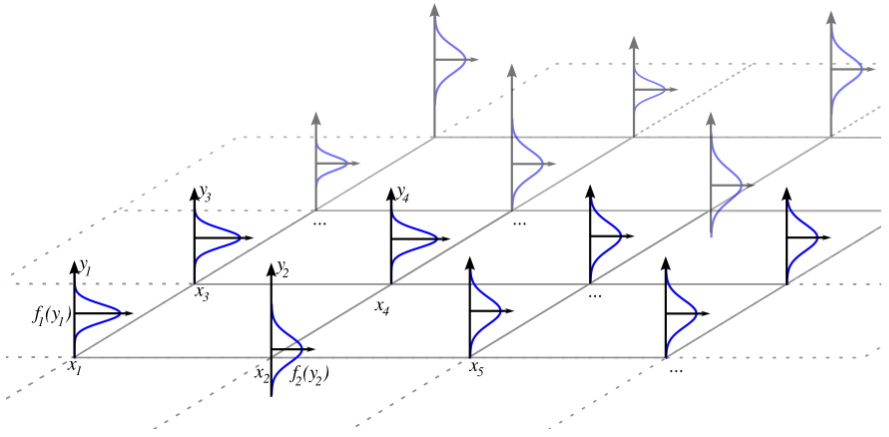
\includegraphics[width=0.95\textwidth]{figures/uncertain_gaussian_field.png}
  \end{center}
  \caption{Illustration of an uncertain field with a Gaussian probability density function at every sample point (from \cite{pothkow2015modeling})}
  \label{fig:uncertain field example}
\end{figure}

For similar reasons why continuous data is available mostly in discrete form, the probability density function (PDF) associated with every sample point is in practice rarely given as the actual function, but rather as sampled values. 
In the case of this Thesis, these samples stem from multiple \textit{realizations} $\omega \in \Omega$ ($\Omega$ being the sample space, which represents the different samples of the PDF), wich associates every realization with one version of the field: $F: \Omega \rightarrow \mathbb{R}^n$.
With regard to simulations, one realization $\omega$ is associated with a certain set of parameters for a mathematical model. 
Again, the full set of $\Omega$ cannot be realized, so a certain number $m$ of realizations $Z = (\omega_1,\dots,\omega_m) \in \Omega^m$ is used to approximate the PDFs associated with each grid point. 
Connecting this with the terms mentioned in Section~\ref{sec:climate research}: The set of fields $F(Z)$ is called \textit{ensemble}, while each field $F(\omega_i), i \in {1,\dots,m}$ is the $i$th \textit{member} (or \textit{realization}) of said ensemble. \cite{vietinghoffdiss}  
% With $x_i \in \D, i \in {1, 2, \dots, M}$ (the approximation of $D$ in Equation~\ref{eq:continous data}), 


\section{Empirical Orthogonal Functions}
\label{sec:eof}


\subsection{Overview}

\acf{eof} analysis, also known as geographically weighted \ac{pca} or Proper Orthogonal Decomposition \cite{vietinghoffdiss}, was first introduced to the field of turbulence and fluid dynamics in the late 60s. The goal was to reduce turbulent flow to a limit number of deterministic functions to explain the structure of the flow by showing coherent structures that are otherwise hard to find and define \cite{weiss_tutorial_2019}. Currently, it \enquote{is among the most widely and extensively used methods in atmospheric science} \cite{hannachi_empirical_2007}. 
One of its goals is to reduce the usually very high dimensionality of atmospheric data and can be used to link certain modes/patterns to the physics/dynamics of the analyzed system.  
\acp{eof} are a statistical procedure to decompose spatio-temporal data into two components: On the one hand orthogonal spatial patterns, on the other hand corresponding uncorrelated temporal coefficients, representing the activity of their corresponding pattern in certain time steps \cite{hannachi_empirical_2007, vietinghoffdiss}. 
The naming of the components is far from being consistent: The spatial patterns are also called spatial modes, PC loadings, \acp{eof} or even sometimes PCs, while the temporal coefficients are also named principal components (PCs), \ac{eof} amplitudes or \ac{eof} (expansion) coefficients \cite{hannachi_empirical_2007}. 
So as a formula, a spatio-temporal field $X(t, s)$ (e.g. a sea level pressure field over time mentioned in Section~\ref{sec:nao}) can be described as

\begin{equation}
  X(t, s) = \sum^{M}_{k=1} c_k(t) u_k(s)
  \label{eq:eof decomposition}
\end{equation}

with $M$ being the number of modes/patterns and  $c_k$ the $k$th temporal coefficients and $u_k$ the spatial pattern \cite{hannachi_empirical_2007}. 

This could be achieved with multiple kinds of decomposition, but \ac{eof} tries finding new sets of variables ($c_k(t)$ and $u_k(s)$ from Equation~\ref{eq:eof decomposition}) that each capture a maximum possible amount of variance/variability of the original dataset. 
So the first of $M$ modes captures the most variance, the second one the second most and so on. 
To give a practical example: The patterns shown in Figure~\ref{fig:nao eap} show the first two spatial patterns of \ac{psl} data, the \ac{nao} and \ac{eap} (in the formula those would be $u_1(s)$ and $u_2(s)$). 
The temporal coefficient is basically a float value for each time step, indicating how active the pattern is ($c_1(t)$ and $c_2(t)$ for \ac{nao} and \ac{eap}, respectively). 
This value is shown for all winter seasons in Figure~\ref{fig:naoindex_comparison}, second row. 
A positive value indicates that the \ac{psl} is dominated by the pressure low in the north and pressure high in the south, a negative value the opposite. 
The underlying can then be (approximately) reconstructed by using $x \leq M$ modes/EOFs (e.g. it could be approximated quite well by only using the dominant modes of \ac{nao} and \ac{eap}). 

\subsection{Mathematical Derivation and Computation of \acp{eof}}

The goal of this Section is to give an overview of the mathematical origins of \acp{eof} based on the work of \citeauthorwork{hannachi_empirical_2007} as well as their actual practical computation. 
For a more in depth history and derivation, please refer to \cite{hannachi_empirical_2007} and their references, while \citeauthorwork{weiss_tutorial_2019} gives a great hands-on tutorial on POD/\acp{eof} and their interpretation and computation. 

As already explained, the starting point of \acp{eof} is usually a spatio-temporal field $X(t, s)$ defined on a Grid $G$ over $n$ time steps, for example the precipitation analyzed in this Thesis. 
The value at each grid point at geographical location $s_j$ and time $t_i$ is given as $x_{ij}$, with $i = 1, ..., n$  and $j = 1, ..., p$.  
The first step is usually to remove the climatology of the dataset to turn it into anomaly maps. 
The climatology is usually defined as the temporal mean $\bar{x}$ of the analyzed datachunk, so 
\begin{align}
  \bar{x}_i = \frac{1}{n} \sum^{n}_{k=1} x_{ki} \\
  \bar{x} = (\bar{x}_1, ..., \bar{x}_p)^T .
  \label{eq:climatology}
\end{align}

So the values of anomaly maps $x'_{ij}$ at each grid point are given as the departure of $X$ from its climatology: 



\begin{equation}
  x'_{ij} = x_{ij} - \bar{x}_j \\
  \label{eq:anomaly map elements}
\end{equation}

And so the final anomaly map $X'$ is: 
\begin{equation}
  X' = \begin{pmatrix}
x'_{11} & x'_{12} & \cdots & x'_{1j} \\
x'_{21} & x'_{22} & \cdots & x'_{2j} \\
\vdots & \vdots & \ddots & \vdots \\
x'_{i1} & x'_{i2} & \cdots & x'_{ij}
\end{pmatrix}
  \label{eq:anomaly map}
\end{equation}

% Since from here on only anomaly maps are considered in the derivation and calculation of \acp{eof}, the $'$ gets omitted and $X$ stands now for the anomaly data.  
The first usual step for generating \acp{eof} is the covariance matrix defined by 

\begin{equation}
  S = \frac{1}{n} X'^T X' 
  \label{eq:covariance map}
\end{equation}

This covariance matrix with the values $s_{ab}$ with $a,b = 1, \cdots, p$ contains the covariance of any grid point with any other grid point over the time. 
To find \acp{eof} means determining a unit length direction $u = (u_1, \cdots, u_p)$ that explains the most variability. 
This problem is therefor equivalent to the solution to the eigenvalue problem, so finding all the eigenvectors ($\equiv$ \acp{eof}) and their eigenvalue. Which means that the vector $u$ multiplied by the covariance matrix $S$ is equivalent to the multiplication with a scalar $\lambda^2$ (the eigenvalue):  

\begin{equation}
  Su = \lambda^2 u
  \label{eq:eigenvalue problem} 
\end{equation}

So to find the $k$th \ac{eof} of a Covariance matrix, the eigenvectors $u$ are sorted by the (largest first) value of their corresponding eigenvalue $\lambda^2$. 
The primary (or dominant) \ac{eof} the first in this order, the secondary \ac{eof} the second and so on. 
The variance $v_k$ of the original dataset associated with the $k$th \ac{eof} can then be calculated with: 

\begin{equation}
  v_k = \frac{\lambda^2_k}{\sum^{p}_{i=1} \lambda^2_i}
  \label{eq:eof variance calculation}
\end{equation}

The temporal coefficients can then in turn be calculated projecting the eigenvectors $u_k$ on the original anomaly map $X'$ with: 

\begin{equation}
  a_{k} = X'u_k
\end{equation}

Together they fulfill the requirements of the decomposition in Equation~\ref{eq:eof decomposition}. 
% So the coefficients in Equation~\ref{eq:eof decomposition}
Note here that the solutions being eigenvectors means that the multiplication by any scalar $\alpha$ (i.e. $\alpha u_k$ and $\alpha^{-1} a_k$) is also a valid solution to the problem. 
This leaves room of choosing scale and direction in a useful way (see Section~\ref{sec:eof_calc} for a practical implementation) \cite{vietinghoffdiss}. 

\subsection{Calculation and Application to the geographical Domain}


Since geographical data is usually given on a regular 2D grid which depicts the earth's surface, the influence of grid point density (same degree resolution is far more sparse in equatorial regions than in the Arctic) need to be corrected with geographical weights. 
Those can be approximated by the square root of the cosine of the respective latitude \cite{hannachi_primer_nodate, vietinghoffdiss} with a similar diagonal matrix as depicted in \cite{hannachi_primer_nodate}: 

\begin{equation}
  W = \begin{pmatrix}
    \cos(\theta_1) & 0 & \cdots & 0 \\
0 & \cos(\theta_2) & \cdots & 0 \\
\vdots & \vdots & \ddots & \vdots \\
0 & 0 & \cdots & \cos(\theta_p)
\end{pmatrix}
  \label{eq:geographical weighting}
\end{equation}
  

Fortunately, there is no need to calculate the covariance matrix and solve the eigenvalue problem. 
Linear Algebra provides a tool called \textit{Singular Value Decomposition} (\ac{svd}), which decomposes any matrix $X$ into three components: 

\begin{equation}
  X = L \Lambda R^T 
  \label{eq:svd definition}
\end{equation}

$L$ contains the left singular vectors, $R$ the right singular vectors and $\Lambda$ a diagonal matrix containing the singular values $\lambda_k$ (as used in Equation~\ref{eq:eof variance calculation} above). 

Now all of the above is used to calculate the \acp{eof} of geographical data by applying \ac{svd} to the matrix (like in \citeauthorwork{vietinghoffdiss}): 

\begin{equation}
  \tilde{X} = \frac{1}{\sqrt{n - 1}} W^{\frac{1}{2}} X' 
  \label{eq:complete data preperation}
\end{equation}


When using \ac{svd} of $\tilde{X}$ with time as the first dimension (like depicted here), the columns of $R^T$ are the \acp{eof} (so $u_k(s)$ of Equation~\ref{eq:eof decomposition}) and the columns of $L$ multiplied with $\sqrt{n - 1}$ are the principal components or \ac{eof} coefficients ($c_k(t)$ in Equation~\ref{eq:eof decomposition}).
As explained above, this result can be scaled, which is explained in detail in Section~\ref{sec:eof_calc}.
\todo{go over this whole section and check everything for being correct!!!!}




  \chapter{MPI GE CMIP6}
\label{ch:dataset}

The Max Planck Institute Grand Ensemble CMIP6 (MPI GE CMIP6) is a Single-model initial-condition large ensemble (in short: SMILE) \cite{olonscheck_new_2023}. 
This means that a single model was run with different initial condiditions but the same external forcings (e.g. greenhous gasses) mutiple times ($\Rightarrow$ ensemble). 
This makes it possible to seperate the internal variability from the responses to the external forcing, enabling researchers to better quantify the consequences of climate change (for example) . 
Additionally it makes the research of extreme weather phenomena (e.g. droughts, floods etc.) more robust in spite of their rare occurences \cite{maher_large_2021}. 
As described in Section \ref{sec:climate}, Coupled models 


The dataset chosen for this project is the \textit{Max Planck Institute Grand Ensemble CMIP6} (from now on MPI-GE CMIP6), presented by \citeauthor{olonscheck_new_2023} \cite{olonscheck_new_2023}. 
The reasons for choosing this dataset are manifold:

\begin{enumerate}
  \item It uses the latest (6th) phase of the Coupled Model Intercomparison Project (CMIP6)
  \item Compared to its predecessor (MPI-GE \cite{maher_max_2019}) it provides high frequency output (6 hour intervals vs. monthly means), which enables taking short-lived weather events and structures (e.g. atmospheric rivers) into account which would be lost in the calculation of the mean
  \item 
\end{enumerate}


This section should explain what datasets are available and why I chose the MPI-GE CMIP6 \cite{olonscheck_new_2023}

Maybe but the comparison table from \cite{olonscheck_new_2023} here and expand it a bit. 



  \chapter{Related Work}

\section{Climate simulation datasets}

General infos from \cite{mpige}:

\begin{itemize}
  \item 
	
\end{itemize}

\subsection{RCP Scenarios}

% \subsection{Questions arising about using climate simulation datasets}
% 
% \begin{itemize}
%   \item How many ensemble members are needed for a correct assessment?
%   \item How to sort them out? Random?
%   \item 
% \end{itemize}

\subsection{MPI-GE - The Max Planck Institute grand Ensemble}

General information about the future scenarios (all based on the \textit{rcp85} dataset available to me on the DKRZ cluster, I just assumed its the same for other scenarios. Maybe need to confirm this):

\begin{itemize}
  \item \textbf{Time}: The time axis is  compromised of 1128 values, which count the days since 01.01.2005. The first one is ~380, so it actually starts somewhere in 2006, and all of those values are roughly 30 days apart. This axis is part of every dataset, all stored as floats.
  \item \textbf{Lat}: Vector of 96 Float Elements ranging from roughly -88 to 88. Results in a resolution of 1.875° in North-South direction.
  \item \textbf{Lon}: Vector of 192 Float Elements ranging from roughly 0 to 358. Results in a resolution of 1.875° in East-West direction. 
  \item \textbf{Pressure Level}: Is given for each dataset and consists of 26 Floats, ranging from 10 to 100,000. 
  \item \textbf{Eastward/Northward Wind}: Given as Floats in the unit of $ms^{-1}$ per \textit{(lat, lon, time, plev)}. Each compromises the wind direction in one orthogonal direction. Eastward wind directory is named \textit{ua}, northward \textit{va}  
  \item \textbf{Specific Humidity}: Specific humidity is given as a float without value. Reason is the unit is actually kg moisture per kilogramm air, which cancels out in the end. Is given for each \textit{(lat, lon, time, plev)}. Directory name: \textit{hus}
	
\end{itemize}



In \cite{mpige} there is much information available:




\subsection{CMIP5 - Coupled Model Intercomparison Project}

In \cite{taylor2012overview_cmip5}


\section{Precipitation Literature}

\subsection{Saisonality in Precipitation variability}


The work of \citeauthor{precipitation_seasonality}

\section{Means of moisture transport}

\subsection{vertically integrated water vapor transport}

As proposed by \citeauthor{AProposedAlgorithmforMoistureFluxesfromAtmosphericRivers} in \cite{AProposedAlgorithmforMoistureFluxesfromAtmosphericRivers}, one way of measuring moisture ($p$) transport is by vertically integrating over the different pressure levels the zonal and meridional fluxes $\overline{pu}$ and $\overline{pv}$. 

An example of using this method can be found in \cite{Ayantobo2021IntegratedMT} with many more references why this method is working well for these kinds of approaches. 

Also this paper lists some other methods of moisture transportation which are also used:

\begin{enumerate}
  \item integrated water vapor distributions (see \cite{gimeno2014atmospheric_rivers_review})
  \item the lagrangian approach
  \item stable oxygen isotope investigation
\end{enumerate}

\subsubsection{Usages of IVT and differences}

In \cite{ralph2017dropsonde} they used a vector field of the IVT: $\int_{p_{low}}^{p_{max}} qV dp$, where $p$ is the pressure level, $q$ is the humidity and $V$ the horizontal vector.

In \cite{sousa2020north} they used a scalar field based on the euclidian norm of the vector field used by \cite{ralph2017dropsonde}.


In \cite{Ayantobo2021IntegratedMT} they also used the euclidian norm on a similar field like \cite{ralph2017dropsonde} to measure the impact of  ENSO on south-chinese weather.
% They used it to measure the moisture and displayed the first graphics of the work, illustrating how an IVT map looks at a drought and during a flood.
% Also maps of the mean IVT during each months, displaying the intense raining/wet summers and dry winters

\subsection{Moisture Budget}

\citeauthor{atmos13101694} showed in their report \cite{atmos13101694} the directions of moisture flux on the continent borders based on the big ERA5 reanalysis.
They measure the moisture based on a equation called the \textit{Moisture Budget}, which is based on multiple Faktors: 



It seems related to the IVT the other authors used, but utilizes the gradient and some other differences. The complete formula is:

$$
\frac{1}{g} \frac{\delta}{\delta t} \int^{P_s}_0 q dp = - \nabla \cdot \frac{1}{g} \int^{P_s}_0 (qv) dp + E - P
$$

With: 

\begin{enumerate}
  \item $p$ is the pressure, $P_s$ is the surface pressure
  \item $q$ is the specific humidity
  \item $v$ is the horizontal wind vector
  \item $E$ is the evaporation
  \item $P$ is the Precipitation
\end{enumerate}


In the actual analysis they used mostly other metrics:


\begin{enumerate}
  \item Vertically integrated Moisture Convergence (\textit{VIMC}): It is basically the gradient of the specific moisture in the air times the Wind vector
  \item $P$ is the precipitation 
  \item $E$ is the evaporation
\end{enumerate}

Furthermore they evaluateded the correlation between the moisture transport and the precipitation variability, which correlate to a significant extent.

\section{Pattern analysis}

\subsection{Empirical Orthogonal Functions}

See \cite{hannachi2007eof_review} for a big overview of EOF in atmospheric science.

See \cite{Ayantobo2021IntegratedMT} for an similar approach as we plan it, except it only focuses on the past.
They 

  \chapter{Design}
\label{ch:design}



  \chapter{Evaluation}
\label{ch:evaluation}


  \chapter{Conclusions and Future Work}
\label{ch:conclusions}

\section{Conclusions}
\label{sec:conclusions}



\section{Future Work}
\label{sec:FutureWork}



% This ensures that the subsequent sections are being included as root
% items in the bookmark structure of your PDF reader.
\bookmarksetup{startatroot}
\backmatter

  \begingroup
    \let\clearpage\relax
    \glsaddall
    \printglossary[type=\acronymtype]
    \newpage
    \printglossary
  \endgroup

  \printindex
  \printbibliography

\end{document}
